\chapter{Voltage regulation}\label{ch:voltageRegulation}
%**********************************************

%**********************************************
\section{Introduction} \label{sec:voltIntro}
%**********************************************

Given a 9 $V_{DC}$ battery, a voltage regulator is required to reduce the voltage level to 5 $V_{DC}$, as this is the level required by the operational amplifiers used in the rest of the circuit. Two voltage regulators were considered: the LM7805 linear regulator as well as the LM2595 switchmode regulator, which were both analysed with regards to efficiency and noise by means of calculations and simulations. According to the literature, the linear regulator does not really output noise, but has low power efficiency of around $50\%$ for input-output of 9 $V_{DC}$ and 5 $V_{DC}$\cite{lm7805}. The switchmode regulator can provide power efficiency of around $85\%$, but outputs a considerable amount of noise\cite{lm2595}. With the aforementioned in mind, both of the regulators were simulated (Section \ref{sec:voltDesign} to determine the best trade-off between low noise and efficiency. Resistor and capacitor configurations were determined according to the respective datasheets \cite{lm7805} \cite{lm2595}.

%**********************************************
\section{Design} \label{sec:voltDesign}
%**********************************************

	\subsection{Linear Regulator} \label{sec:linreg}
\begin{figure}[h]
    \centering
    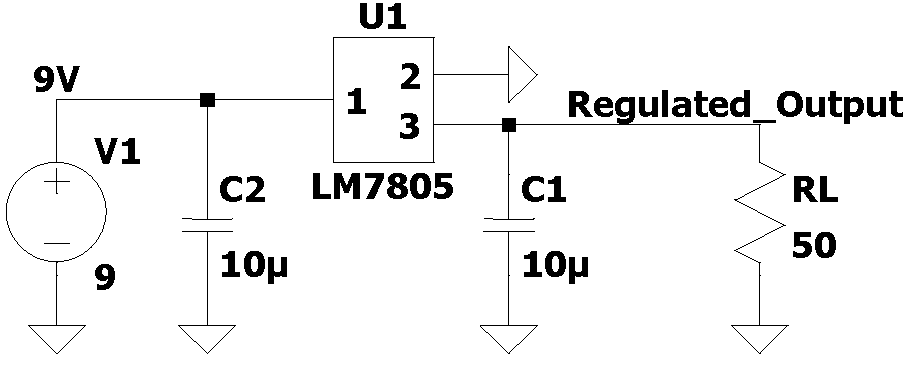
\includegraphics[width = 0.8\textwidth]{Figures/LR.pdf}
    \caption{Linear Voltage Regulator}
    \label{fig:LR}
\end{figure}

The LM7805 chip is shown in Figure \ref{fig:LR}, as well as the required peripheral circuit, which was obtained from the datasheet \cite{lm7805}. For testing purposes, a \SI{50}{\Omega} load was connected to the regulator, drawing \SI{100}{mA}. Measurements are discussed in section \ref{sec:comp}.


	\subsection{Switchmode Regulator} \label{sec:smreg}
\begin{figure}[h]
    \centering
    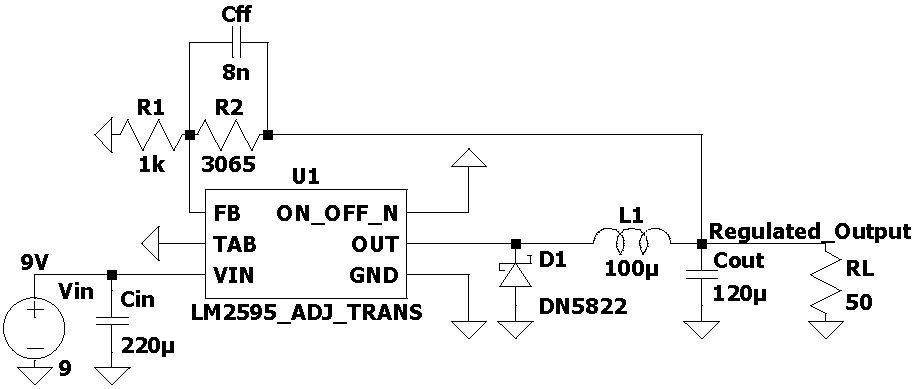
\includegraphics[width = 1\textwidth]{Figures/SM.pdf}
    \caption{Switchmode Voltage Regulator}
    \label{fig:SM}
\end{figure}

The LM2595 chip is shown in Figure \ref{fig:SM}, built into the required peripheral circuit. Capacitor and inductor values are as shown, and were obtained from the datasheet \cite{lm2595}. Resistor values were calculated as follows:

$$\mathrm{V}_{\mathrm{OUT}}=\mathrm{V}_{\mathrm{REF}}\left(1+\frac{\mathrm{R}_{2}}{\mathrm{R}_{1}}\right) \quad \text { where } \mathrm{V}_{\mathrm{REF}}=1.23 \mathrm{V}$$

Selecting $\mathrm{R_1}$ as \SI{1}{\kilo\Omega}, with $\mathrm{V_{out}}$ as \SI{5}{\volt} gives $\mathrm{R_2}$ as \SI{3065}{\Omega}. For testing purposes, a \SI{50}{\Omega} load was connected to the regulator, drawing \SI{100}{mA}. Measurements are discussed in section \ref{sec:comp}.


	\subsection{Voltage Regulator Comparison} \label{sec:comp}
The input and output power measurements are displayed in table \ref{tab:compvreg}.
\begin{table}[h]
        \centering
        \footnotesize
        \caption{Comparison of Voltage Regulators}
         \begin{tabular}{c@{\qquad}rrrrr}
          \toprule
             & $I_{in}$ [mA] & $I_{out}$ [mA] & $P_{in}$ [mW] & $P_{out}$ [mW] & $\eta$ [\%] \\
          \midrule
          LM7805 	& 105.06 	& 100.05 	& 945.54 	& 500.55 	& 52.93\\
          LM2595 	& 57.54 	& 99.65 	& 517.86 	& 496.6 	& 95.89\\
          \bottomrule
        \end{tabular}
     \label{tab:compvreg}
\end{table}

Comparing the efficiency of the respective regulators, it is clear that the switchmode regulator is considerably more efficient. However, simulation results in a settling time of \SI{1.24}{ms}, which is quite slow. Furthermore, the switchmode regulator creates noise levels of up to 950 $\mathrm{mV_{pp}}$ in the output, as can be seen in figure \ref{fig:smnoise}. This is a problem, as the large gain of the differential amplifier, which is fed by the voltage regulator, will result in the noise levels to increase in magnitude and become prevalent in the output. Considering all of the above, the linear regulator was selected for the design, despite being less efficient, as it provides an almost instantaneous settling time, coupled with negligible amounts of noise.

\begin{figure}[h]
    \centering
    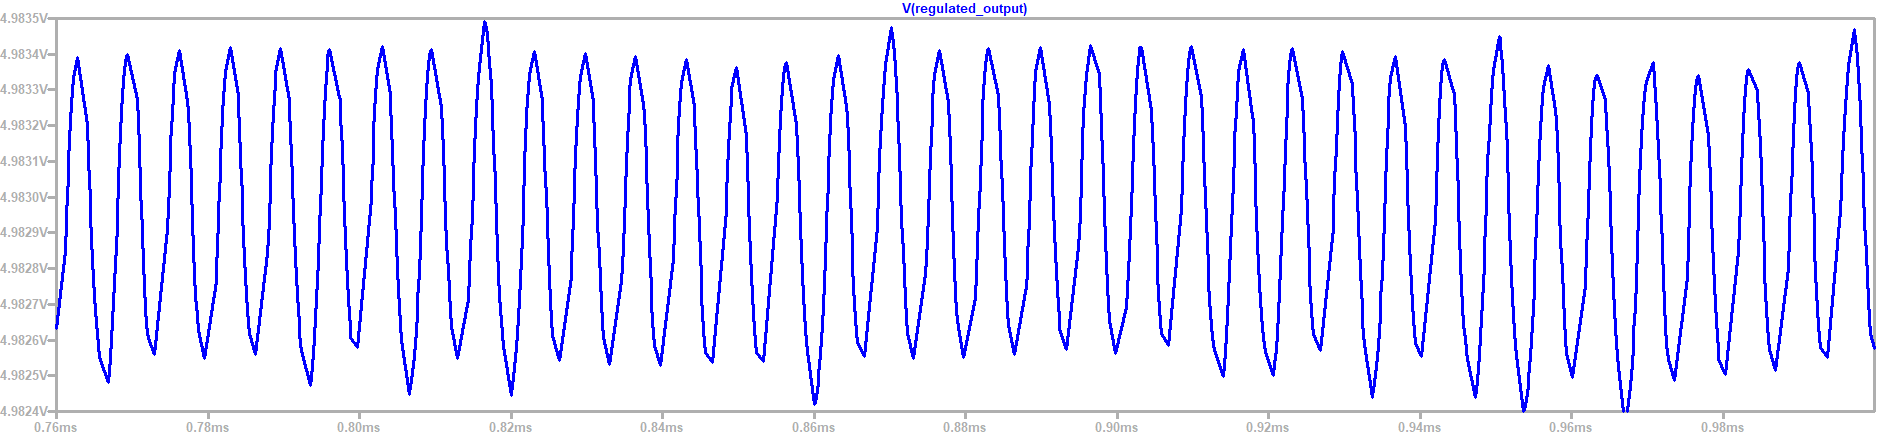
\includegraphics[width = 0.8\textwidth]{Figures/smnoise}
    \caption{Switchmode Voltage Regulator Output}
    \label{fig:smnoise}
\end{figure}

\textbf{More vreg calcs, Voltage reg power calcs before sim?}

%**********************************************
\section{Results} \label{sec:volt_results}
%**********************************************

%\begin{figure}
% \footnotesize
% \centering
%    \begin{subfigure}[]{0.55\textwidth}
%              \centering
%  		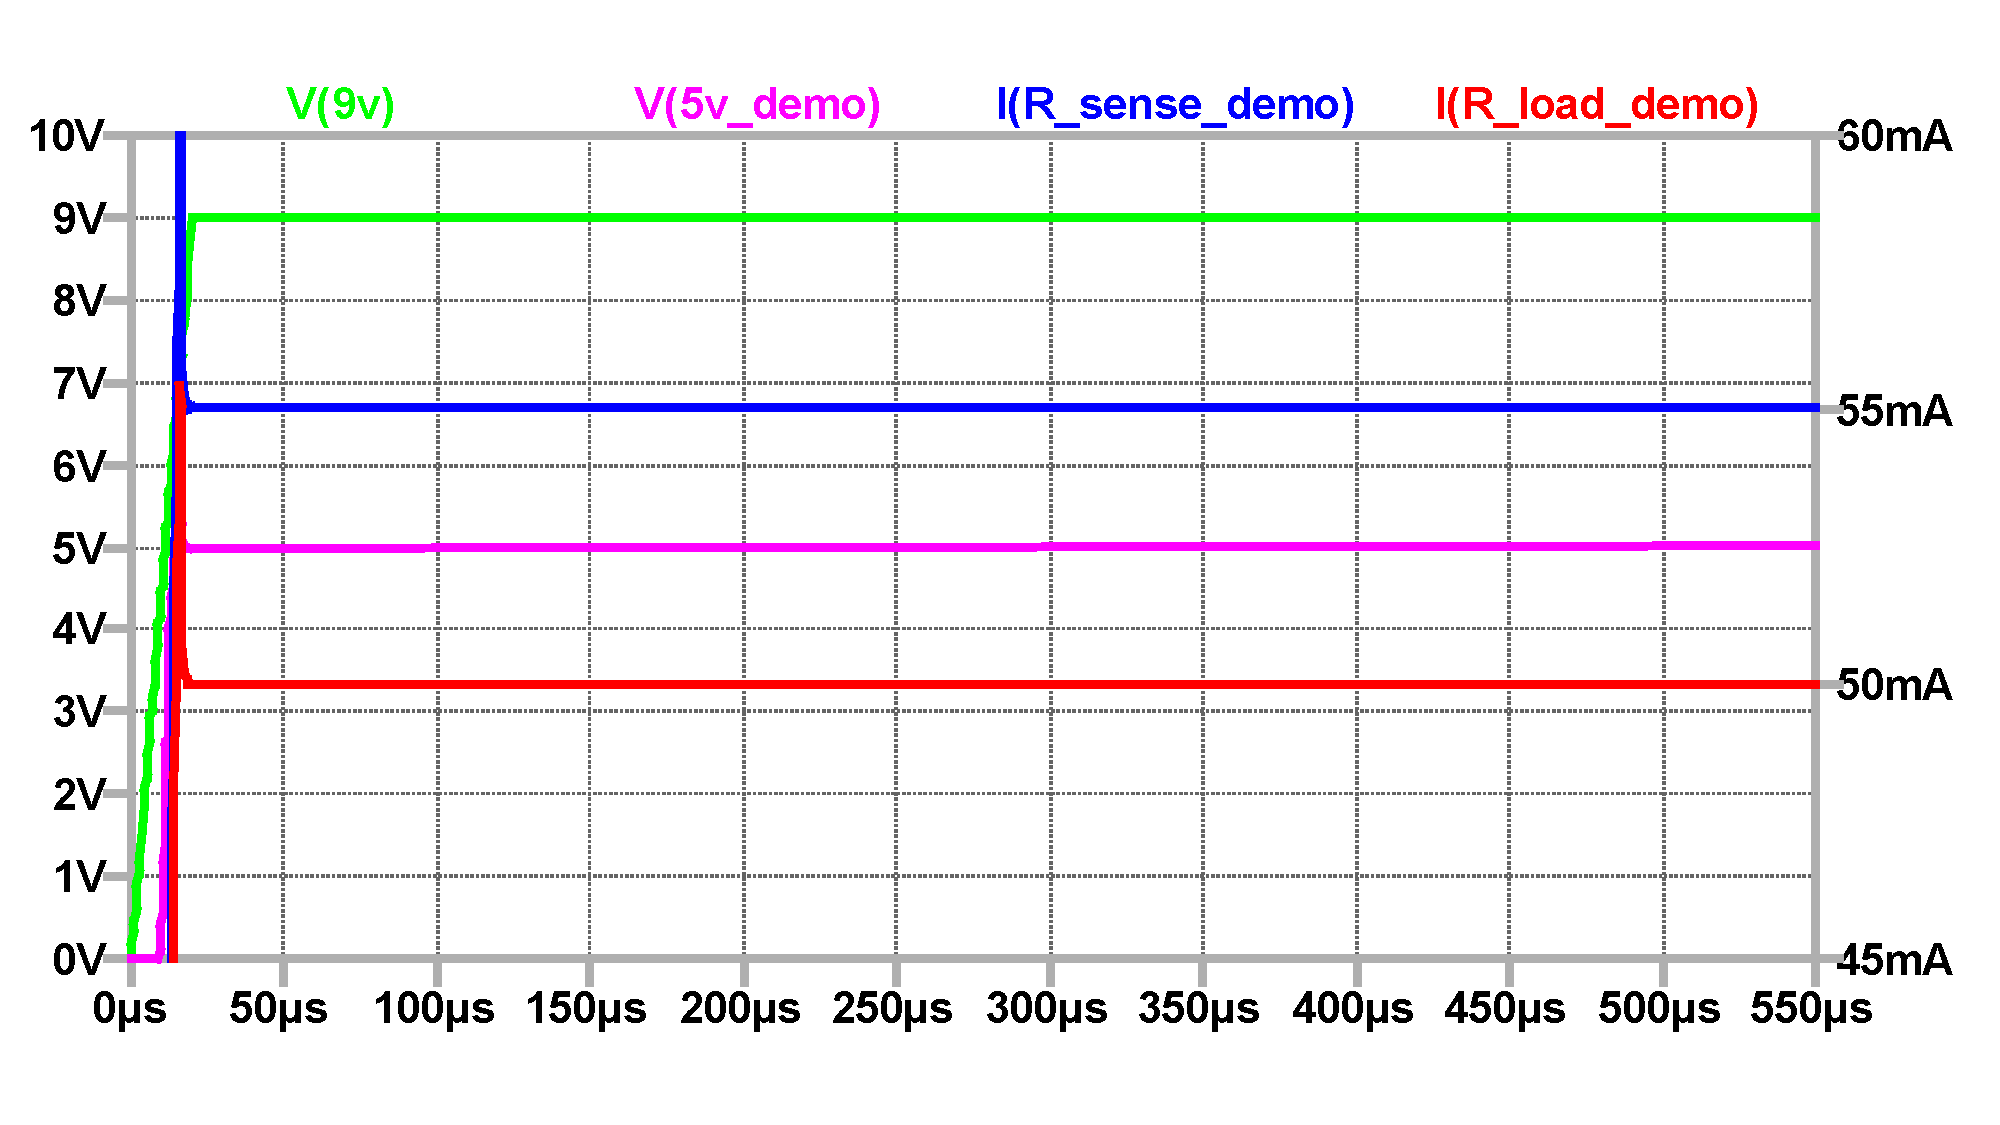
\includegraphics[width=1\linewidth]{./Figures/E344_VoltRegulator.pdf}
%		    \caption{} \label{subfig:pwr_simu_rect}
%     \end{subfigure}
%     \begin{subfigure}[]{0.4\textwidth}
%             \centering
%  		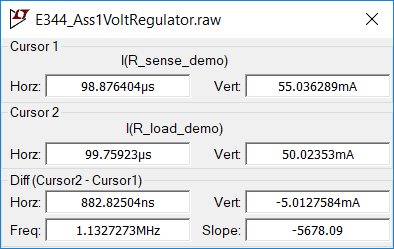
\includegraphics[width=1.0\linewidth]{./Figures/Screengrab2}
%		   \caption{ } \label{subfig:pwr_meas_rect}
%     \end{subfigure}
%    \begin{subfigure}[]{0.55\textwidth}
%              \centering
%  		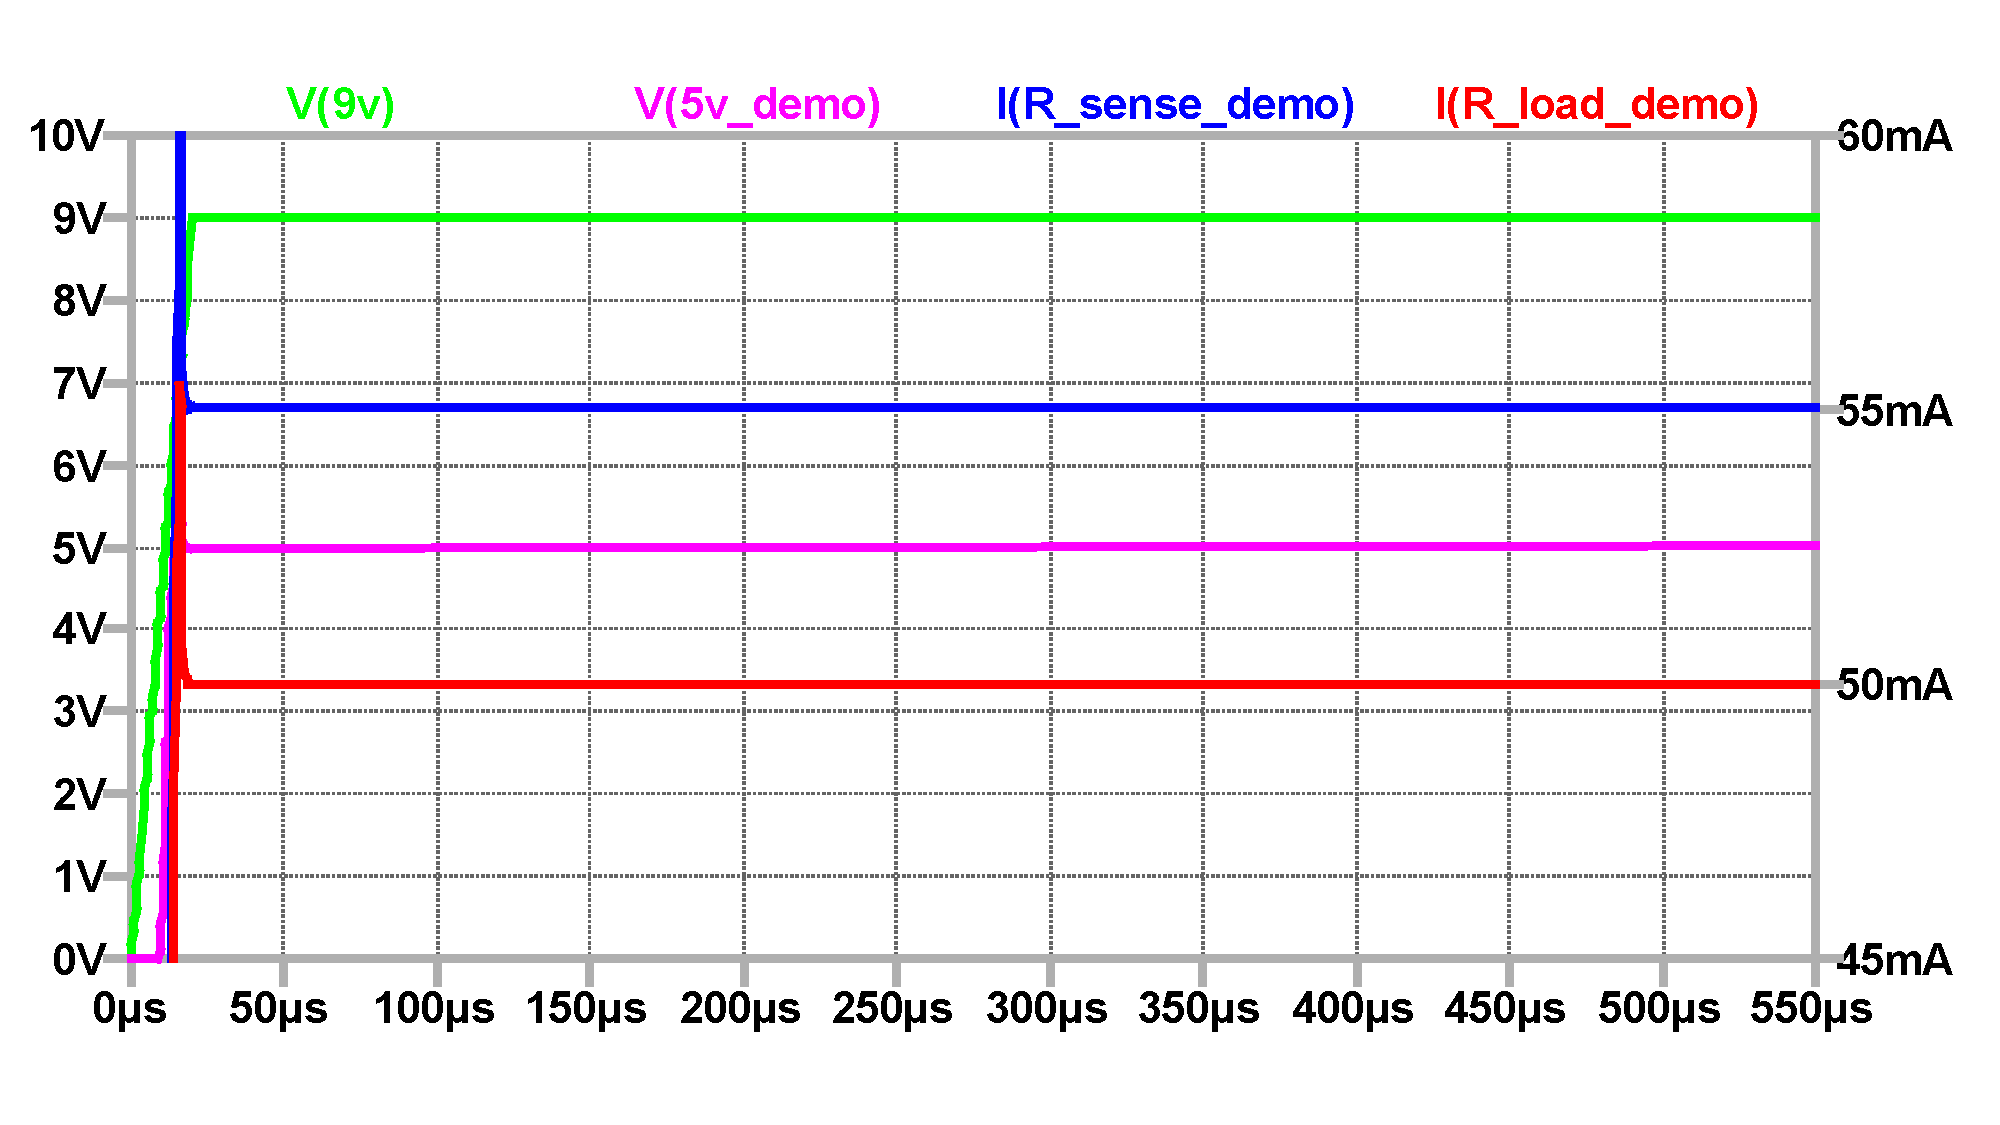
\includegraphics[width=1\linewidth]{./Figures/E344_VoltRegulator.pdf}
%		    \caption{} \label{subfig:pwr_simu_rect}
%     \end{subfigure}
%    \begin{subfigure}[]{0.4\textwidth}
%              \centering
%  		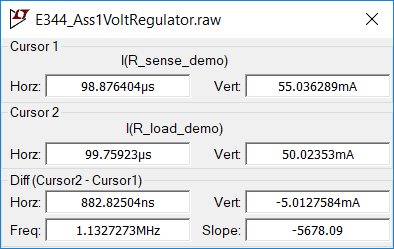
\includegraphics[width=1\linewidth]{./Figures/Screengrab2}
%		    \caption{} \label{subfig:pwr_simu_rect}
%     \end{subfigure}
%   \caption[\textcolor{red}{I am the short caption that appears in the List of Figures list}]{Voltage regulation, comparing the linear and switchmode regulators... (a)  Blah blah. (b)  Blah blah.  (c)  Blah blah. (d) Blah blah.   As far as possible, please put input(s) and output(s) on the same plot rather than on separate plots. Based on the datasheet of XXXX in \cite{WebsiteOpAmp}}
%    \label{fig:simulation_results_box}
% \end{figure}

In this section, you want to demonstrate, by means of referring to simulation results, using the designed circuit, how your circuit behaves as you designed it in Section \ref{sec:voltDesign}. Present and report on your simulated results in Figure \ref{fig:simulation_results_box} Be absolutely sure that the text and information in your report are readable. 

You can use screengrabs or photos of the oscilloscope, or download the CSVs and plot them as PDFs using Matlab, Excel or similar. 
You can also use tables, example of which are presented in Tables \ref{tab:table1} and \ref{tab:table2}.


\begin{table}
        \centering
        \footnotesize
        \caption{Example of a simple table.}
         \begin{tabular}{c@{\qquad}rrrr}
          \toprule
             & 2017 & 2018 & $\Delta_{Abs}$ & $\Delta_{DiD}$\\
          \midrule
          A & 9,868      & 10,399 & +5 & -11\\
          B & 10,191     & 10,590 & +4 & -12\\
          \bottomrule
        \end{tabular}
     \label{tab:table1}
\end{table}


\begin{table}
         \centering
        \footnotesize
        \caption{Example of another table.}

         \begin{tabular}{c@{\qquad}rrrr}
          \toprule
          \multirow{2}{*}{\raisebox{-\heavyrulewidth}{Schools }} & \multicolumn{2}{c}{Total energy used}& \multicolumn{2}{c}{Change}\\
          \cmidrule{2-5}
            & 2017 & 2018 & $\Delta_{Abs}$ & $\Delta_{DiD}$\\
            & [kWh] & [kWh] & [\%] & [\%] \\
          \midrule
          A & 9,868      & 10,399 & +5 & -11\\
          B & 10,191     & 10,590 & +4 & -12\\
          \bottomrule
        \end{tabular}
     \label{tab:table2}
\end{table}


%**********************************************
\section{Summary}\label{sec:temp_summary}
%**********************************************
Concluding, it has been shown that both regulators behave as expected, but that the levels of noise present in the switchmode regulator make it unsuitable for the design at hand, as input signals, and thus the noise as well, will be amplified to levels of noise in the output signal that are unacceptable for an ADC input. This choice was made despite the fact that the switchmode regulator is approximately 40\% more efficient than the linear regulator, influenced thereby that the total current drawn is still very low. However, it should be noted that the current drawn should be re-evaluated after the rest of the components have been connected to the regulator, in order to make sure that the current draw requirement still is met.


